\section{\textbf{Method}}
By searching through various scientific articles, thermochromic data for a material in the 
form of either a complex dielectric constant $\varepsilon (\omega,T)$ or complex refrective index 
$N(\omega, T)$ was found. By the use of a program called \textsc{Engauge Digitizer} graphically represented
data, such as graphs or plots, could be extracted for use in numerical calculations. \textsc{Engauge Digitizer}
is a open source digitizing software and can be found on
http://digitizer.sourceforge.net/.
It can convert image files of type \texttt{.bmp, .jpeg} or other,
containing a graph or a map, into numbers. The conversion from graphical to numerical data
is obtained through defining three 
points the image, e.g. the origin, largest x-value and largest y-value for a function y = f(x),
which define the x,y-axes together with their scale. 
The target data can be marked automatically or manually, depending on the quality of the image. 
The data can then be exported to a spreadsheet and used in numerical calculation.
\\
\\
Of the extracted data, only the data from Kang et al. \cite[p.~3]{Kang2012} were used,
for reasons being that these were the only data that overlapped with the relevant data from
the material database for \textsc{GranFilm}. Kang et al. provided data for the dielectric constant
of VO$_2$ as functions of energy, with one graph per temperature. The data were then interpolated in 
order to provide $\varepsilon(E,T)$ for $E \in [0.5eV,4.0eV], T \in [25^{\circ}C, 80^{\circ}C]$.
%Due to lacking overlap between the already included material data in \textsc{GranFilm} and the new extracted
%data, only data from Kang et al. \cite[p.~3]{Kang2012}, containing the dielectric constant of 
%VO$_2$ have been used. 
It would be interesting to include data from several thermochromic materials. However, the
ease of the data extraction with \textsc{Engauge Digitizer} dependens on the quality and 
degree of overlap of the functions and could be very tedious. 
Further extractions have therefore not been prioritized. \textbf{??Should I say this, or is it best to leave it out???}
\\
\\
The material data input to be read by \textsc{GranFilm} must however be on a specific form. 
\textsc{GranFilm} requires a complex refractive index $N$ as a discrete function of energy or wavelength. 
The real and imaginary values of $N$ must be given for each point of its domain. In addition, the 
values of the domain must consist of equdistant values. The resulting data through the use of 
\textsc{Engauge Digitizer} is not equidistant and because the real and imaginary data is usually
extracted from different image files, their values do not correspond to the same discrete domain. 
\\
\\
Because of this mismatch between the extracted image data, using \textsc{Engauge Digitizer}, 
and the input file format of \textsc{GranFilm}, some conversion had to be done.
The data was converted to the form $N(E,T) = n(E,T) + ik(E,T)$ as a function of equidistant
energy steps, with [$E$]=eV, and could now be fed into \textsc{GranFilm}.
\\
\\


\subsection{Choice of parameters}
Due to the quasistatic approximation where it was assumed that the layer thickness or the size
of the particles should be negligible compared to the wavelength of the incident light $R \ll \lambda$. Here
$R$ is the radius of the island.
In addition, the separation of the particles should be so small that they are excited by the same incident
field, i.e. the lattice constant $L \ll \lambda$.
Since the simulation computes for optical wavelengths down to about about 350nm, the simulation
was run for $r \in [10$nm$,15$nm$]$ with $L = 45$nm.

\subsection{Simulation}
%
\begin{figure}[h!]
    \centering
    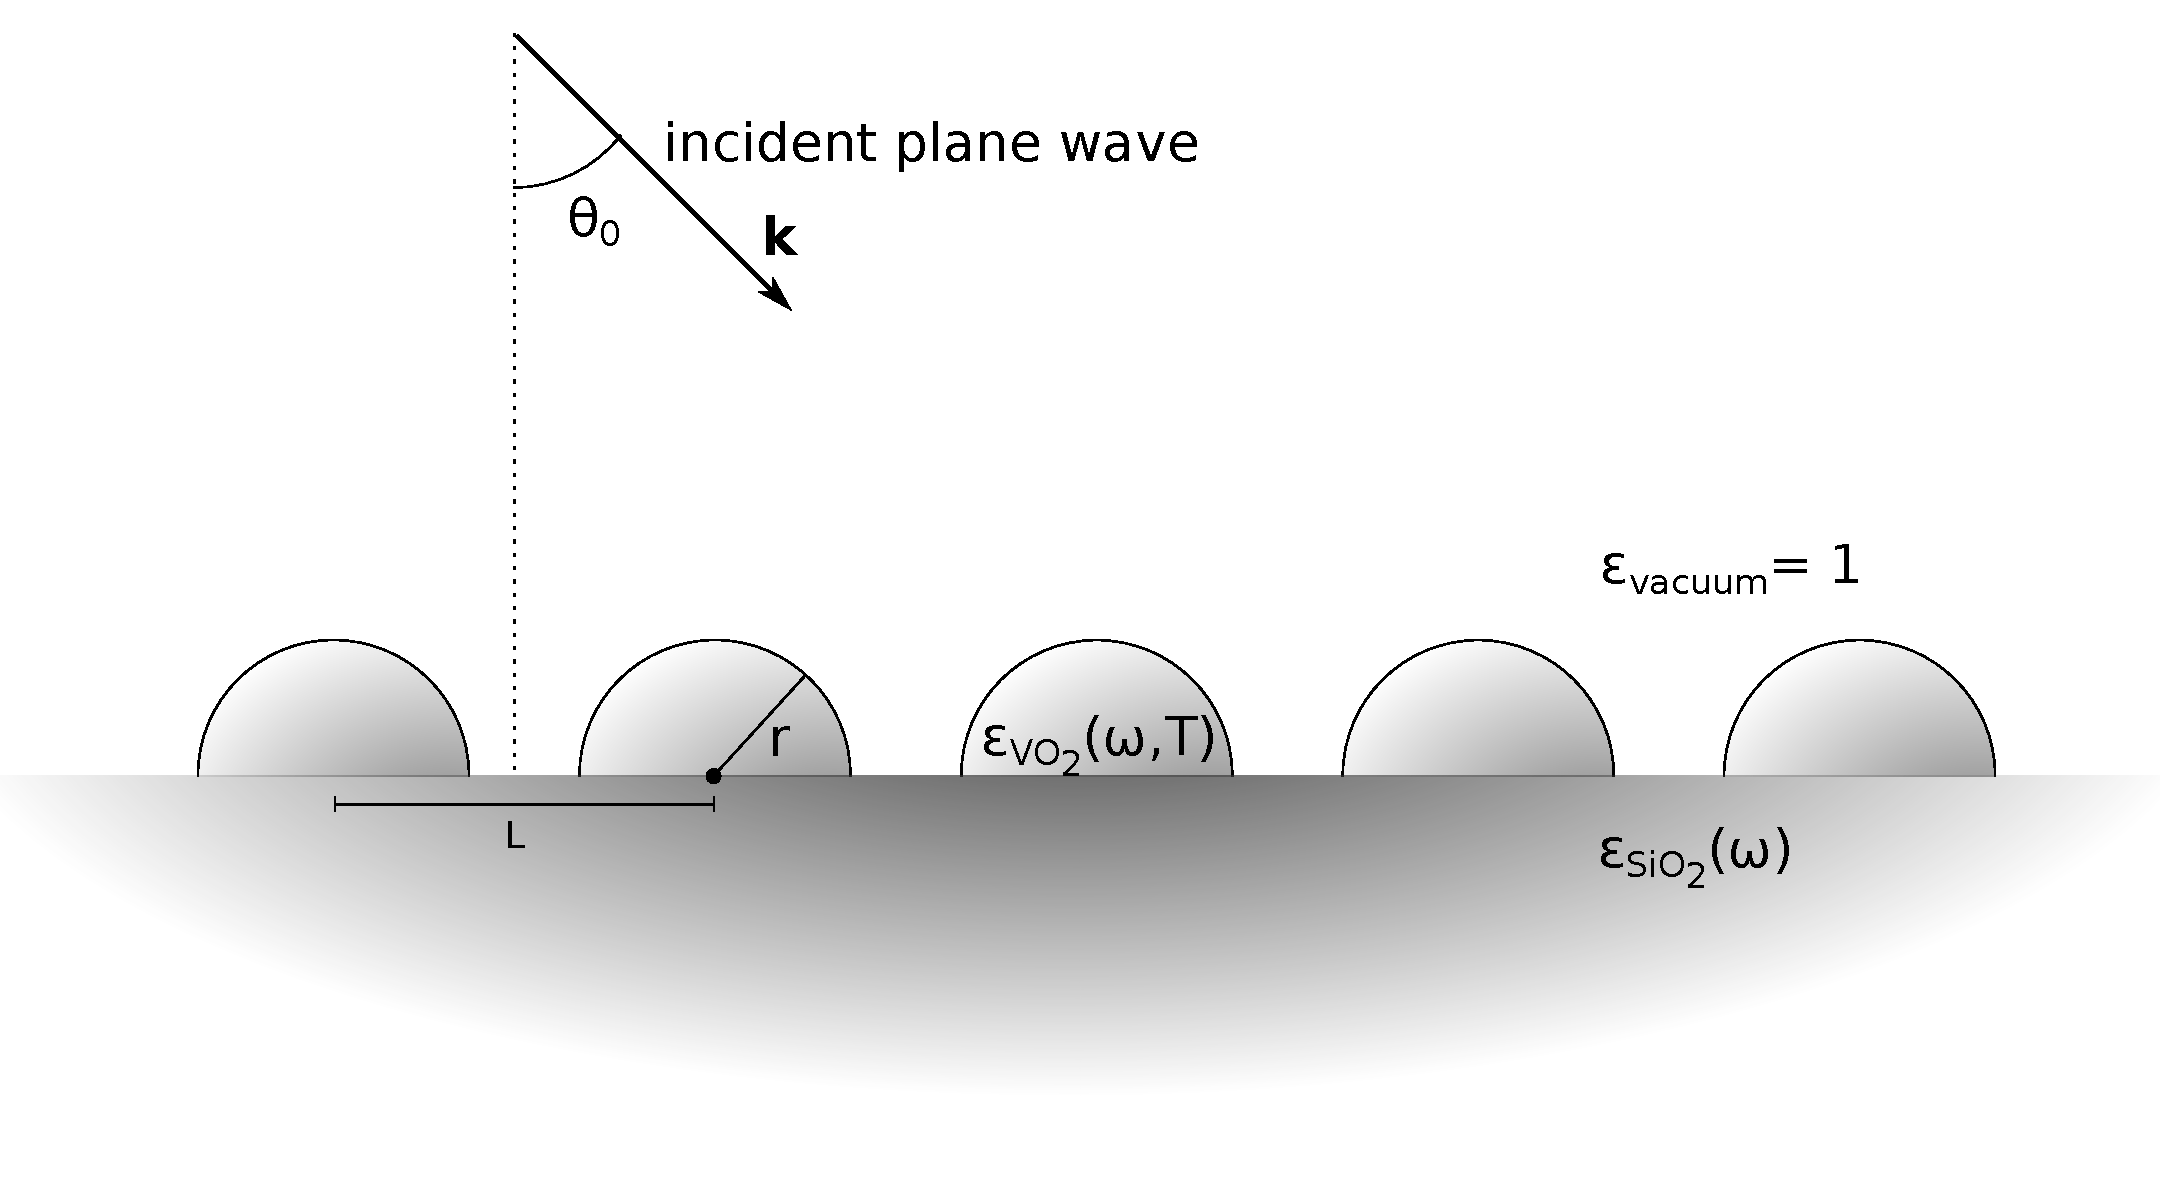
\includegraphics[width=0.9\textwidth]{Figures/simulation1.pdf}
    \caption{
       The simulation was run for a VO$_2$ particles supported by a SiO$_2$ substrate. The surrounding
       medium was set to vacuum with dielectric constant $\varepsilon = 1$. VO$_2$ is assumed to
       be the only material displaying temperature dependent behavior.
    }
    \label{fig:simulationFigure}
\end{figure}
%
Because of the response of the granular layer in the visible region and due to the reports on the
unattractive colors of VO$_2$ thin films \cite{Blackman2009}, the color was investigated
using the free software \textsc{ColorPy}. \textsc{ColorPy} is a Python package that convert physical
descriptions of light, such as light intensities, into RGB colors. The resulting colors are only approximate
due to both the model and the monitor used to display the colors \cite{colorpy}. 
But because the uncertainties of the
extracted data using \textsc{Engauge Digitizer}, the analysis is primarily qualitative and the
resulting colors is assumed to be adequate. \textbf{?!?!?Er dette greit å skrive?!?!?!?!?}
%?????????????????????????????????????????????????????????????????????????????????????????

\textbf{REMEMBER TO COMMENT OUT THIS (choise of parameters):}
\begin{itemize}
   \item talk about the corresponding intervall we're simulating (the energy range and the corresponding
      wavelength range).
   \item Then talk about how large sphere sizes we're then allowed to use.
   \item relate this up towards the mentioned thicness mentioned by the sources and comment on it.
   \item (...)can not use the thin optimal film layer thickness between 40-90nm as mentioned by 
      Kamalisarvestani et al. \cite{Kamalisarvestani2013} and Blackman et al. \cite{Blackman2009}.
   \item the region of interest based on the introduction is the visible range ($\in \sim $[400,800nm] 
      or [3-4eV,1eV]) and the IR range ($\in \sim $[800nm,10$^5$-10$^6$nm] or [1eV,10$^{-3}$eV]) 
      \cite[p.~11]{Smith}
\end{itemize}

\begin{thebibliography}{9}

   \bibitem{Kang2012}
   Kang M, Kim SW, Ryu JW, Noh T.
   Optical properties for the Mott transition in VO2.
   AIP Advances 2012;2,012168 \textbf{Er dette greit? Finner ikke sidetall osv.}

   \bibitem{Smith}
   Smith GF, King TA, Wilkins D.
   Optics and photonics: an introduction (second edition).
   Wiley 2007.

   \bibitem{colorpy}.
      Kness M,
      ColorPy -- A python package for handling physical descriptions of color and light spectra.
      2008: %Do i need some university stuff here? seems like it's only a private person.
      http://markkness.net/colorpy/ColorPy.html
      (23. September 2015).
      %My interp. of webpage source: 
      %Authors, title, stuff behind(like university?) year ,link (date of site access)
\end{thebibliography}



